\documentclass[12pt, oneside, a4paper]{article}

\usepackage[utf8]{inputenc}     % kodowanie na UTF-8

%##############################################################################
% Global variables
\newcommand{\globalFullAuthor}{Maciej Sypień}          % Pełna nazwa autora pracy
\newcommand{\globalShortAuthor}{M. Sypień}         % Autor - zwięzła forma wydruku
\newcommand{\globalFullTitle}{Zaawansowana egzemplifikacja teorii zależności XYZ}
\newcommand{\globalFullUniversity}{Uniwersytet Ekonomiczny w Krakowie}   % Pełna nazwa uniwersytetu
\newcommand{\globalShortUniversity}{UEK}  % Skrócona nazwa uniwersytetu
\newcommand{\globalDepartment}{Wydział Zarządzania}  % Wydział
\newcommand{\globalKeywords}{nauka, praca, latex, zadanie}
\newcommand{\globalDegreeprogramme}{Informatyka Stosowana}  % Kierunek studiów
\newcommand{\globalDocumentType}{Zadanie semestralne}  % Typ pracy dyplomowej
\newcommand{\globalVersion}{1.0.0}  % wersja pracy - przydatne przy systemie kontroli wersji

%##############################################################################
% Additional packages
\usepackage[polish]{babel}
\usepackage{csquotes}
\usepackage[T1]{fontenc}           % ,,europejski'' układ fontów (Cork)
%\usepackage[OT4,plmath]{polski}   % Zestaw czcionek
\usepackage{times}                 % Times - Czcionki wektorowe
\usepackage{graphicx}              % Wstawianie grafiki
\usepackage{geometry}              % 
\usepackage[usenames]{color}       % Palety kolorów zdefionwanych
\usepackage{fancyhdr}              %
%\usepackage{titlesec}              %
%\usepackage{tocloft}               %
\usepackage{amsmath}               % Moduł matematyczny AMS
\usepackage{amsfonts}              % pakiet czcionek AMS
\usepackage{amsthm}                % Definicje matematyczne AMS
\usepackage[dvipsnames,svgnames]{xcolor}    % Zestaw kolorów             
\usepackage{indentfirst}           % uzyskanie wcięcia przy pierwszym akapicie
\usepackage{nameref}               % pakiet referencji do pełnych nazw rozdziałów
\usepackage{subcaption}
\usepackage{array}
\usepackage{footnote}
\usepackage{lipsum}              % pakiet odpowiedzialny za `lorem ipsum`
\usepackage{indentfirst}   % uzyskanie wcięcia przy pierwszym akapicie
\usepackage[
  font=small,
  format=hang,
  labelformat=simple,
  justification=justified,
  labelsep=colon]{caption}       % pakiet dla podpisów np: dla lstlintings
\usepackage{nameref}       % pakiet referencji do pełnych nazw rozdziałów
\usepackage{enumerate}
\usepackage{multirow}      % pakiet dla łaczenia wierszy w tabelach
\usepackage[framemethod=tikz]{mdframed}     % pakiet zastępujący mało modalny \fbox
\usepackage{listings}      % pakiet dla kodów zródłowych
\usepackage[dvipsnames]{xcolor}

%##############################################################################
% Dodanie komendy dla caption + source
\newcommand*{\captionsource}[2]{%
  \caption[{#1}]{%
    #1%
    \\\hspace{\linewidth}%
    {Źródło:} #2%
  }%
}

%##############################################################################
% Wydruk kodu/tekstu w ramce
\newmdenv[
    skipabove=0.2cm,
    skipbelow=0,
    nobreak=true]{outputbox}


%##############################################################################
% Zdefiniowanie nowego, dodatkowego jezyka
% \lstdefinelanguage{LaTeX}{
%   keywords={\textbf, \$, \$\$, \int, \noindent,},
%   keywordstyle=\color{blue}\bfseries,
%   ndkeywords={class, export, boolean, throw, implements, import, this},
%   ndkeywordstyle=\color{darkgray}\bfseries,
%   identifierstyle=\color{black},
%   sensitive=false,
%   comment=[l]{\%},
%   morecomment=[s]{/*}{*/},
%   commentstyle=\color{purple}\ttfamily,
%   stringstyle=\color{red}\ttfamily,
%   morestring=[b][\color{ForestGreen}]\$,
%   morestring=[b][\color{ForestGreen}]\$\$
% }

%##############################################################################
% Zdefiniowanie nowego, dodatkowego stylu
\lstdefinestyle{LaTeX2e}{
  language=[LaTeX]TeX,
  keywordstyle=\color{Red},
  basicstyle=\ttfamily,
  alsoletter={\#},
  morekeywords={chapter},
  morestring=[b][\color{ForestGreen}]\$,
  morestring=[b][\color{ForestGreen}]\$\$
}


\lstdefinestyle{Bash}{
  language=Bash,
  keywordstyle=\color{MidnightBlue},
  basicstyle=\ttfamily,
  alsoletter={-},
  sensitive=false,
  morekeywords={sudo, wget, chmod, dpkg, git},
  %literate={\$}{{\textcolor{MidnightBlue}{\$}}}1
  %         {-}{{\textcolor{MidnightBlue}{-}}}1
  %         {~}{{\textcolor{MidnightBlue}{\textasciitilde}}}1,
}


%##############################################################################
% Ustawienie opcji dla wyświetlania kodów źródłowych
% Wiecej: pakiet listings s. 26
\lstset{
  literate={ą}{{\k{a}}}1
           {ć}{{\'c}}1
           {ę}{{\k{e}}}1
           {ó}{{\'o}}1
           {ń}{{\'n}}1
           {ł}{{\l{}}}1
           {ś}{{\'s}}1
           {ź}{{\'z}}1
           {ż}{{\.z}}1
           {Ą}{{\k{A}}}1
           {Ć}{{\'C}}1
           {Ę}{{\k{E}}}1
           {Ó}{{\'O}}1
           {Ń}{{\'N}}1
           {Ł}{{\L{}}}1
           {Ś}{{\'S}}1
           {Ź}{{\'Z}}1
           {Ż}{{\.Z}}1,
  %language=[LaTeX]TeX,
  style=LaTeX2e,
  captionpos=t,
  tabsize=2,
  frame=lines,
  keywordstyle=\color{MidnightBlue},
  commentstyle=\color{OliveGreen},
  stringstyle=\color{Red},
  numbers=left,
  numberstyle=\small,
  breaklines=true,
  showstringspaces=false,
  basicstyle=\ttfamily,
  emph={label},
}


%##############################################################################
% Zdefiniowanie własnych nazw dla poszczególnych definicji, twierdzeń itp
\theoremstyle{plain}
\newtheorem{thm}{Twierdzenie}[section]
\newtheorem{lem}[thm]{Lemma}
\newtheorem{prop}[thm]{Założenie}
\newtheorem*{cor}{Wniosek}

\theoremstyle{definition}
\newtheorem{defn}[thm]{Definicja}
\newtheorem{conj}{Przypuszczenie}[section]
\newtheorem{exmp}{Przykład}[section]

\theoremstyle{remark}
\newtheorem*{rem}{Remark}
\newtheorem*{note}{Note}

%##############################################################################
% Ustawienie linkowania dokumetu oraz elementów wyświetlania pdfa
% (Rozdział 4.7.4 z latex w 129 minut)
\usepackage{hyperref}
\hypersetup{
  unicode=true,
  pdfencoding=unicode,
  pdfencoding=auto,
  pdftoolbar=true,        % show Acrobat’s toolbar?
  pdfmenubar=true,        % show Acrobat’s menu?
  pdffitwindow=false,     % window fit to page when opened
  pdfstartview={FitH},    % fits the width of the page to the window
  pdftitle={\globalFullTitle},          % title
  pdfauthor={\globalFullAuthor},        % author
  pdfsubject={\globalDocumentType},    % subject of the document
  pdfcreator={\globalFullAuthor},       % creator of the document
  pdfproducer={\globalFullAuthor},      % producer of the document
  pdfkeywords={\globalKeywords}, % list of keywords
  pdfnewwindow=true,          % links in new window
  linktoc=page,               % Ustawienie linków dla bibliografi (none, all, page, section)
  colorlinks=true,            % false: boxed links; true: colored links
  linkcolor=Maroon,             % color of internal links (change box color with linkbordercolor)
  citecolor=PineGreen,        % color of links to bibliography
  filecolor=Maroon,           % color of file links
  urlcolor=MidnightBlue,      % color of external links
}


%##############################################################################
% Definicje własnych, nowych makr

% poniższe makra wymagają pakietu 'xcolor'
\newcommand{\red}[1]{{\color{RedOrange}{#1}}}
\newcommand{\yellow}[1]{{\color{Dandelion}{#1}}}
\newcommand{\green}[1]{{\color{LimeGreen}{#1}}}
\newcommand{\RED}[1]{{\colorbox{RedOrange}{#1}}}
\newcommand{\YELLOW}[1]{{\colorbox{Dandelion}{#1}}}
\newcommand{\GREEN}[1]{{\colorbox{LimeGreen}{#1}}}

%##############################################################################
% Lowercase \nameref = \lnameref
\newcommand{\lnameref}[1]{%
\bgroup
\let\nmu\MakeLowercase
\nameref{#1}\egroup}

% First UpperCase then lowercase = \fnameref
\newcommand{\fnameref}[1]{%
\bgroup
\def\nmu{\let\nmu\MakeLowercase}%
\nameref{#1}\egroup}

% helper for lowercase newcommands
\newcommand{\nmu}{}

%##############################################################################
% Section Author
\makeatletter
\newcommand{\chapterauthor}[1]{%
  {\parindent0pt\vspace2*{-25pt}%
  \linespread{1.1}\large\scshape#1%
  \par\nobreak\vspace*{35pt}}
  \@afterheading%
}
\makeatother

%##############################################################################

\title{
	\LARGE{\globalFullUniversity}\\
	\vspace{0,3cm}
	\Large{\globalDepartment}\\
    \vspace{3cm}
	\Huge{\globalFullTitle}
	\vspace{2cm}
}
\author{\globalFullAuthor}
\date{\today}

%##############################################################################
% Bibliography options
\usepackage[
    style=authoryear, % numeric, alphabetic, authoryear, 
    backend=biber,]{biblatex}
\addbibresource{bibliografia.bib}  % dołączenie plików bibliografii


%##############################################################################
\begin{document}
\nocite{*}     % wszystkie pozycje z bibliografii
\maketitle     % tworzy tytuł + imiona autorów + datę
\vspace{1cm}

\begin{abstract}
Dokument ten prezentuje całkowicie zmyślony przykład zadania domowego, pracy kontrolnej, semestralnej, ect. w~oparciu o system składu tekstu \LaTeX{} wraz z przykładem pliku do zarządzania pozycjami bibliograficznymi.\\ 
Większość treści nie ma większego sensu z uwagi na zastosowanie pakietu \texttt{lipsum} oraz drobnych wycinków moim tekstów.

Praca ma stanowić przykład prostego użycia obrazków, tabel, list wypunktowanych, odnośników do rozdziałów,  odnośników do pozycji bibliograficznych ect. Projekt ten jest wygodnym startem do pisania własnych dokumentów w LaTeXu.
\end{abstract}

\clearpage
\tableofcontents     % wstawia spis treści

\section{Wprowadzenie}
\label{sec:wprowadzenie}

\lipsum[2-3]

\subsection{Definicja zależności XYZ}

\begin{defn}[Zależność X-Y, z~j. ang. \textit{Dependency of XYZ}] 
\lipsum[1]
\end{defn}

\begin{itemize}
\item Morbi;
\item Mecenas;
\item Alinquam;
\item Suscipit;
\end{itemize}

\lipsum[6-8]

\begin{figure}[!h]
\centering
    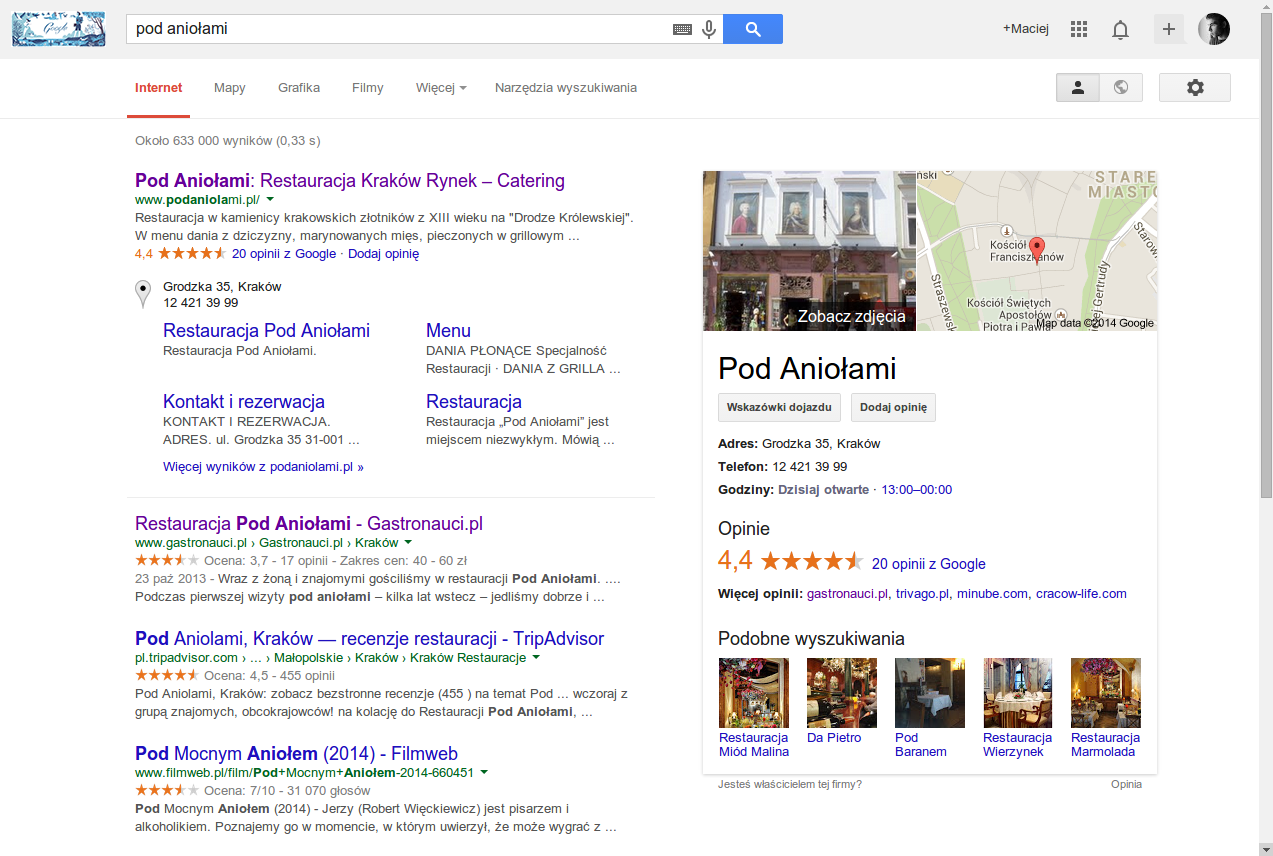
\includegraphics[width=1.0\textwidth]{images/search-result-company-in-google-search-engine.png}
    \captionsource{Wyszukiwanie firmy w~wyszukiwarce Google}{Opracowanie własne.}
    \label{fig:search-result-company-in-google-search-engine}
\end{figure}

%--------------------------------------

\subsection{Rodzaje zależności XY}
\lipsum[6-10] All is according to \parencite{url:zaraz-po-instalacji}.

\begin{figure}[!h]
\centering
\begin{subfigure}{.5\textwidth}
  \centering
  
\includegraphics[width=.4\linewidth]{images/googleplus_color.png}
  \caption{Logo tekstowe}
  \label{fig:google-logo-tekstowe}
\end{subfigure}%
\begin{subfigure}{.5\textwidth}
  \centering
  \scalebox{0.7}
  {
      
\includegraphics[width=.4\linewidth]{images/google-plus-logo.png}
  }  
  \caption{Logo graficzne}
  \label{fig:google-logo-graficzne}
\end{subfigure}
\captionsource{Rodzaje logotypów występujących na witrynie Google+}{\url{https://plus.google.com/}}
\label{fig:logo-google}
\end{figure}

\lipsum[30-33]

\
%\section{Pusta sekcja}

Nic tu jeszcze nie ma.
\section{Teoria zależności QWE w Google}
\label{sec:teoria-zaleznosci-qwe-w-goole}

\begin{figure}[!h]
\centering
\begin{subfigure}{.5\textwidth}
  \centering
  
\includegraphics[width=.4\linewidth]{images/googleplus_color.png}
  \caption{Logo tekstowe}
  \label{fig:google-logo-tekstowe}
\end{subfigure}%
\begin{subfigure}{.5\textwidth}
  \centering
  \scalebox{0.7}
  {
      
\includegraphics[width=.4\linewidth]{images/google-plus-logo.png}
  }  
  \caption{Logo graficzne}
  \label{fig:google-logo-graficzne}
\end{subfigure}
\captionsource{Rodzaje logotypów występujących na witrynie Google+}{\url{https://plus.google.com/}}
\label{fig:logo-google}
\end{figure}

\lipsum[12-14]


%############################################################################

\subsection{QWE, a Google+}
W chwili obecnej tj. 2 kwartale 2014 roku wyszukiwarka Google zajmuję 1 miejsce wśród narzędzi do wyszukiwania informacji w~Polsce (95,59\% udziału rynku), zaraz za nią MSN (2,57\%) oraz Yahoo (0,97\%) \parencite{url:gemius-ranking-silnikow-wyszukiwarek}.

Google będąc największym potentatem rozwiązań wyszukiwania informacji w~internecie na polskim rynku można pokusić się nawet o stwierdzenie że jest niemal monopolistą rynkowym, spychając rywali na wąski margines.

Tak ogromny udział w~rynku zapewnia niemal nieograniczone możliwości kreacji promocji w~sieci. Jednak z~punktu widzenia wolności i~konkurencyjności rynku, ,,wyszukiwarek'' baron dyktuje koszty promocji wszystkim tym, którzy korzystają z~jego produktów --- a jest to niemal całość polskiego społeczeństwa $\sim$96\%. Tak wielki procent udziałów w~rynku, poniekąd zmusza firmy do skorzystania z~oferty Google, jeśli chcą dotrzeć do większości polskich internatów. \\

\lipsum[18-26]

%############################################################################
\subsection{Panel Google+}
Panel Google+ to obszar skupiający w~jednym miejscu kluczowe informacje dotyczące różnych obszarów istotnych w~prowadzeniu firmy w~internecie (tu celowo pomijam użytkownika indywidualnego, ponieważ nie jest on tematem dysputy w~niniejszej publikacji).\\

\begin{figure}[!h]
\centering
    \scalebox{0.21}
    {
        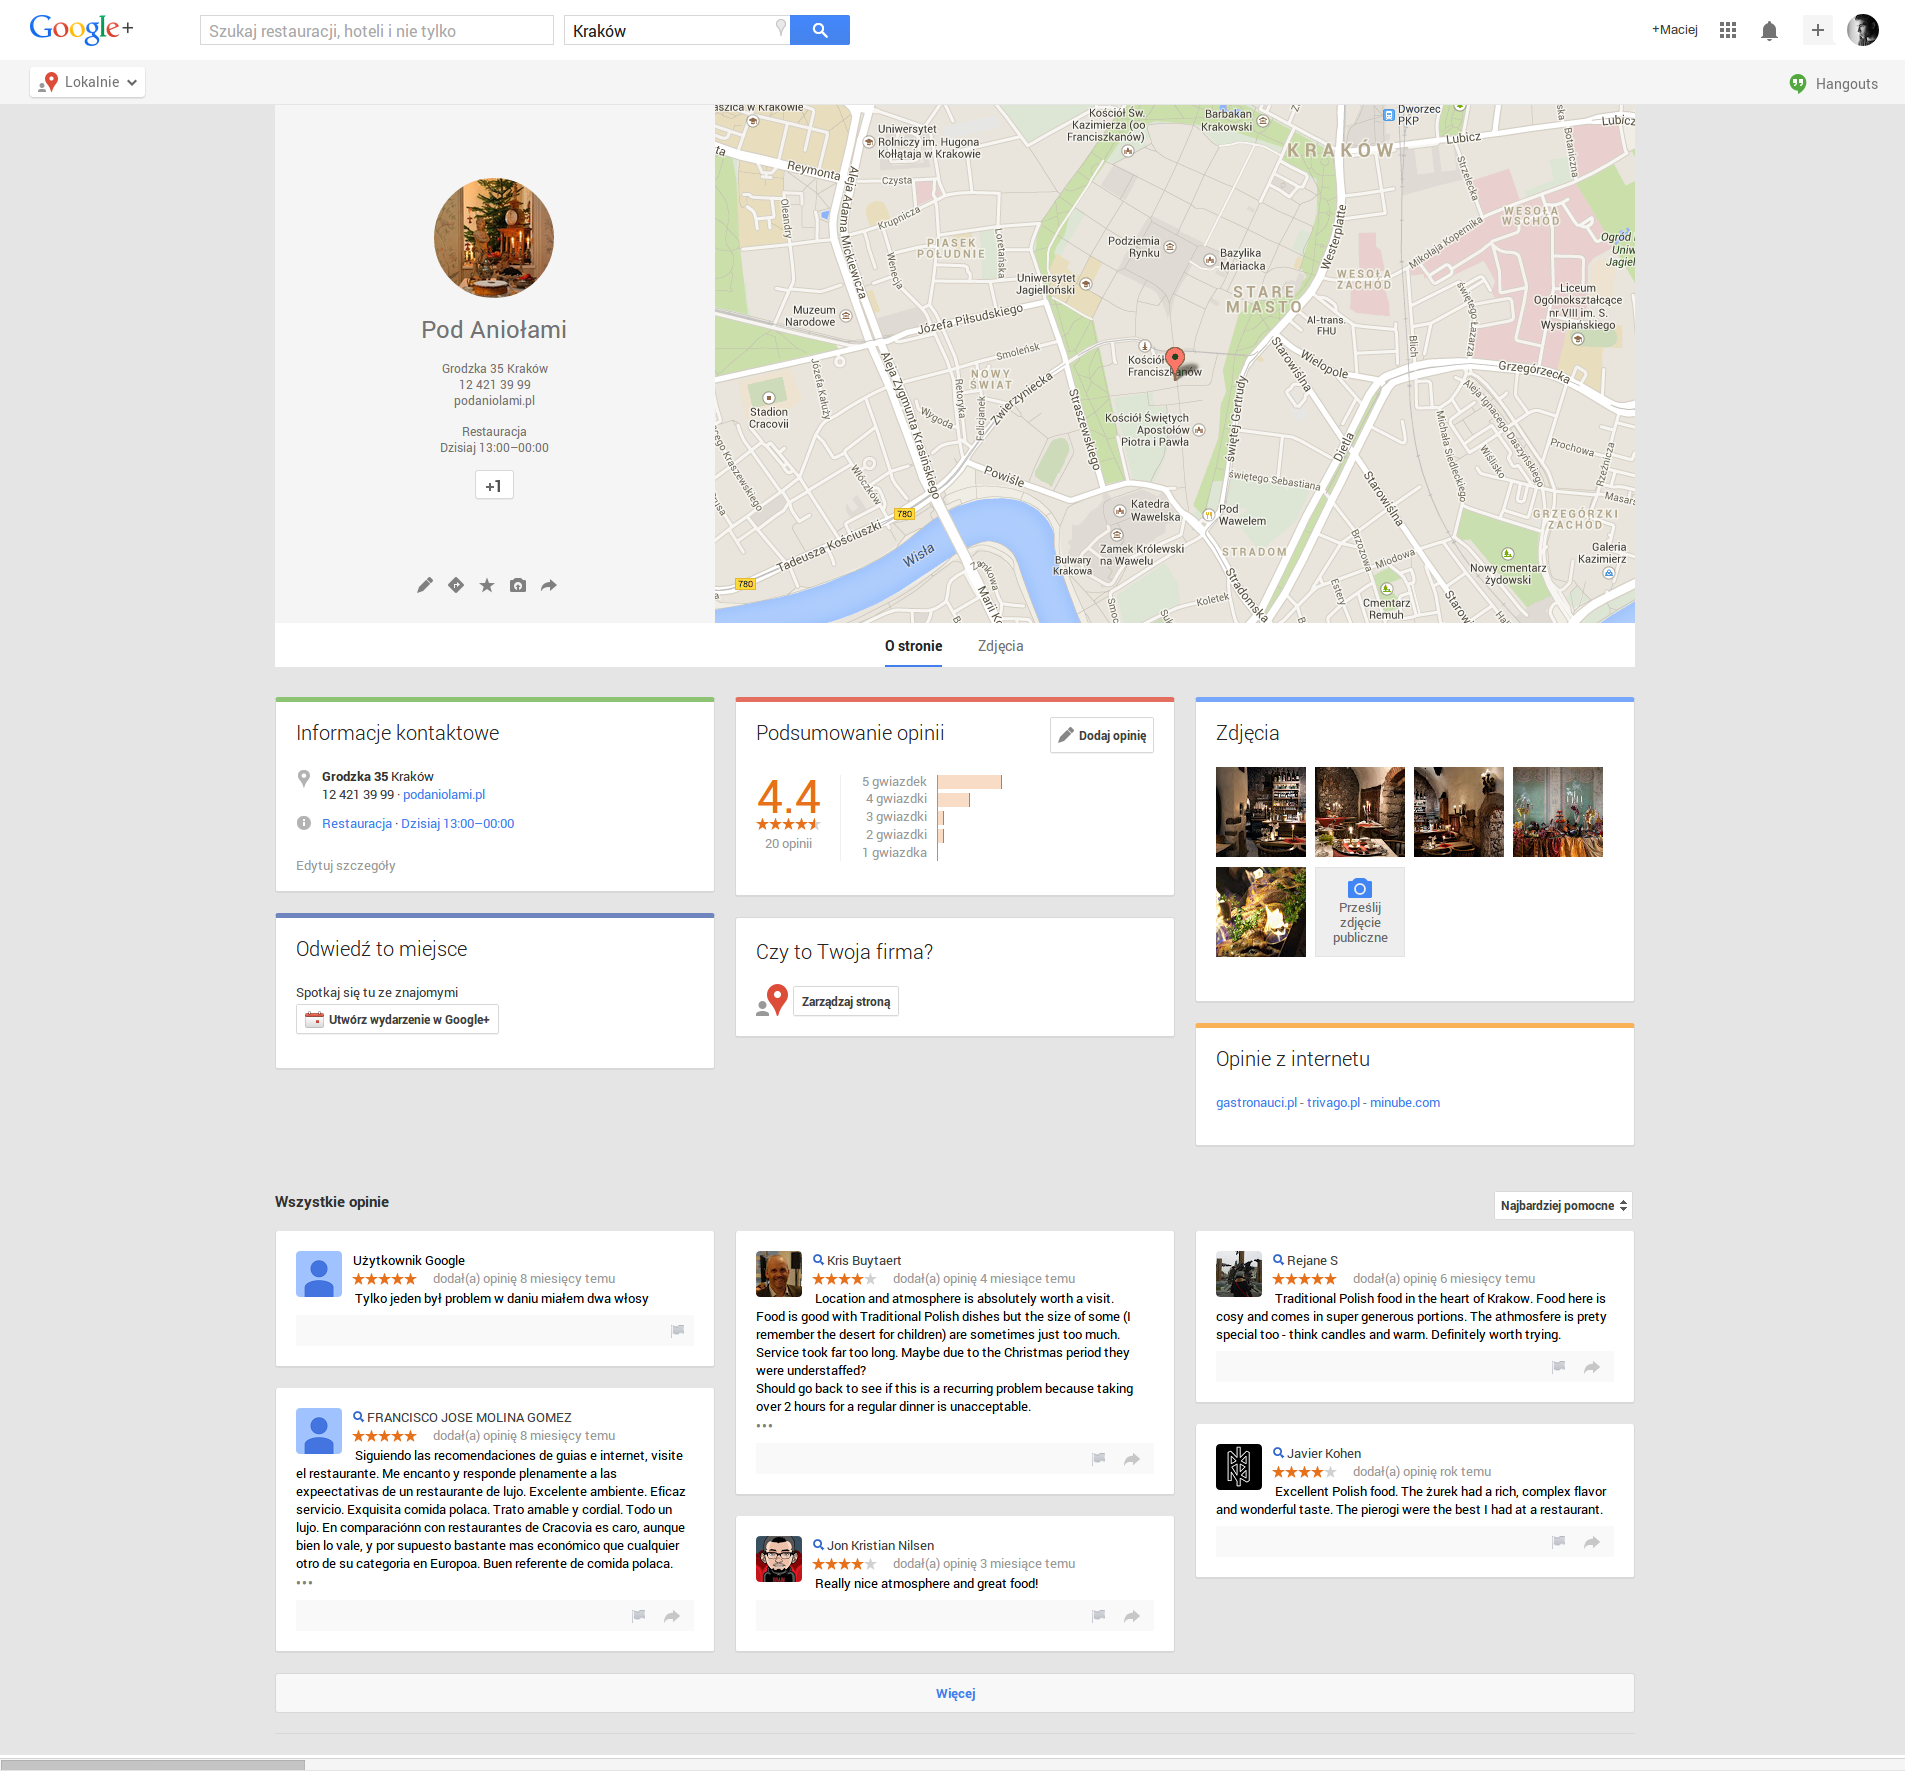
\includegraphics{images/pod-aniolami-google-plus.png}
    }
    \captionsource{Przykładowy profil firmy w~Google+}{Opracowanie własne}
    \label{fig:sample-google-plus-company-profile-page}
\end{figure}

Panel Google+ dostarcza m.in:

\begin{itemize}
\item Możliwość aktualizacji danych firmy w~1 miejscu;

\item Narzędzia sprawdzające kompletność i~zgodność witryny z~wyszukiwarką \mbox{Google};

\item Wyświetlać wpisy innych użytkowników oraz tworzyć własne z~informacjami, zdjęciami i~filmami.

\item Szeroka interakcja z~klientami poprzez budowanie precyzyjnego grona odbiorców oraz udoskonalanie swoich zasobów odpowiadając na opinie użytkowników o firmie/usłudze.

\item Rozmawiać bezpośrednio ,,twarzą w~twarz'' z~klientami dzięki usłudze Google Hangouts (internetowy odpowiednik Skype lub Viber);

\item Przeglądać szeroki zakres różnego typu statystyk dotyczących firmy a w~tym:
    \begin{itemize}
    \item Najpopularniejsze wyszukiwania na temat firmy w~wyszukiwarce Google;
    \item Skąd klienci wyznaczą trasy dojazdu do placówki dzięki usłudze Google Maps;
    \item Sprawdzenie popularności firmy wśród społeczności Google+;
    \end{itemize}

\item Zarządzać reklamami, w~tym także poprzez integrację z~usługą AdWords Express;

\item Mobilność dostarczanych rozwiązań (Smartphone, Tablet, Komputer);
\end{itemize}

%############################################################################
\subsection{Możliwości promocji w~Google+}
\lipsum[80-83]

\begin{exmp}
\label{exmp:latex-table-basic-example-A}
Wyświetlenie podstawowej tabeli otoczonej pojedynczą linią  z każdej strony. \\
\begin{table}[!h]
\centering
    \begin{tabular}{|r|l|}
    \hline
    wiersz1-kolumna1 & wiersz1-kolumna2 \\ 
    \hline
    wiersz2-kolumna1 & wiersz2-kolumna2 \\ 
    \hline
    \end{tabular}
\caption{To jest opis tabeli z przykładu \ref{exmp:latex-table-basic-example-A}}
\label{tab:tab:prosta-tabela-przyklad-A}
\end{table}
\end{exmp}

%############################################################################
\subsubsection{Jak wykorzystać strony Google+ w~biznesie?}
\parencite[s.119]{Brogan12} \lipsum[1]

\begin{itemize}
\item Narzędzia edukacyjnego;
\item Kanału użytkowników;
\item Platformie komunikacyjnej;
\item Centrum medialnemu;
\item Przestrzeni współpracy i~wymiany danych;
\end{itemize}

Każdy z~powyższych przykładów w odwołaniu do całego rozdziału \nameref{} rządzi się swoimi prawami, zaletami i~wadami płynącymi z~prowadzenia określonej struktury profilu. Trudno tu faworyzować konkretne rozwiązanie, ponieważ wybór charakteru wykorzystania profilu winien być świadomy i~równoważny, równoważący bądź uzupełniający wykorzystanie innych kanałów mediów społecznościowych, gdyż każde medium jest swoistą odmianą komunikacji panującej między użytkownikami\footnote{Jeden  z~portali społecznościowych służy jako wymianie wiedzy, drugi jako informator dla lokalnej społeczności, a trzeci może wyłącznie skupiać się na relacjach biznesowych}.

O tym jakie drogi mogą umożliwić promocja w~medium społecznościowym \mbox{Google+} zostanie przybliżona w~kolejnych sekcjach. Przeanalizujemy przykładowe modele i~możliwości płynące z~ich wykorzystania w~różnych sytuacjach.

%############################################################################

\subsubsection{\nmu Wszystko w~jednym miejscu}
\label{subsubsec:wszystko-w-jednym-miejscu}
Dla wielu rekinów biznesu ale i~nie tylko, pewne przysłowie: ,,jak coś jest  do wszystkiego, to jest do niczego'' jest jak najbardziej prawdziwe i~sprawdza się. Jednak w~tym kontekście naszego podrozdziału \lnameref{subsubsec:wszystko-w-jednym-miejscu}, główna strona profilu\footnote{Nota bene profil Google+ inaczej widzi właściciel konta, ponieważ posiada możliwość edycji materiałów na profilu, a nieco odmiennie widzi go klient lub po prostu inny użytkownik portalu google+, który może zaobserwować zwartą kondensacje danych w~postaci prostej przewijanej witryny (aktualnie popularny i~obserwowalny w~internecie model tworzenia witryn www nie wymagający za dużo ,,męczenia się i~klikania'', a jedynie oczekuje od użytkownika przewijanie strony coraz niżej --- taki rozwój stron może być nawet traktowany jako kompensacja rozwoju internetu)}, czyli tak zwany \textit{wall} zawiera wszystkie najpotrzebniejsze informacje dla klienta co widać na rysunku \ref{fig:sample-google-plus-company-profile-page} i~w~tym kontekście powinna być rozpatrywana. Nie jako narzędzie do wszystkiego, chodź za takie może uchodzić ponieważ jest elementem łączącym pozostałe usługi firmy Google przykładowo tj. Hangouts, Google Maps czy AdWords. 

\noindent Jednak oprócz spoiwa różnych usług, którym z~pewnością jest google+, zapewnia również interakcję z~użytkownikiem poprzez umieszczanie postów (w tym tekstu, obrazu, wideo) oraz wydawanie opinii klientów o swoich usługach. 

W głównej mierze ma być miejscem profesjonalnej i~rzetelnej informacji dla klienta. Pytanie tylko czy stosunkowo niedawne wejście na rynek pozwoli poważnemu i~profesjonalnemu Google+ wyprzeć bardziej frywolnego, kierowanego na luźniejsze relację giganta jakim jest Facebook\footnote{Firma Google posiada nieco odmienne założenia społecznościowe dla swoich produktów. Google stawia na wiarygodności i~rzetelność opinii na których można polegać i~równie dobrze szybko odnaleźć (dzięki lepszej współpracy z~własną wyszukiwarką). To są niepodważalne cechy profesjonalizmu dla firm. 
Flagowy produkt firmy Facebook skupia się natomiast na nieco innych założeniach. Mianowicie relacjach międzyludzkich głęboko zakorzenionych w~ludziach jak np.: związkach(słynny status ,,w związku''), przyjaźniach, dzieleniem się informacjami w~bliskim kontakcie z~przyjaciółmi. Model produktu Facebook moim zdaniem ma zastosowanie dla nieco odmiennej grupy firm, niż bardziej uniwersalny Google+, co nie oznacza że zamyka im drogę. Jednak nie wszystko co związane z~firmą, w~oficjalny sposób można wrzucić na Facebook z~racji różnego modelu świadczonych usług obydwu produktów.}.

%############################################################################

\subsubsection{Budowanie społeczności}
Wielokrotnie wspominany profil w~Google+ w~dostarcza wielu różnych usług pomagających w~relacjach społecznościowych.

\begin{figure}[!h]
\centering
    \scalebox{0.25}
    {
        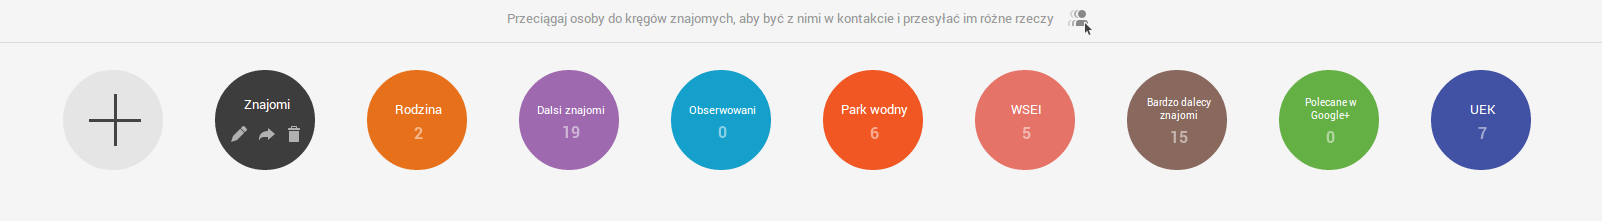
\includegraphics{images/google-plus-circles.png}
    }
    \captionsource{Kręgi w~Google+}{Opracowanie własne}
    \label{fig:google-plus-circles}
\end{figure}

Jedną z~nich są Kręgi (ang. Circles) i~przykładowy zrzut ekranu z~widokiem znajdziemy na rysunku~\ref{fig:google-plus-circles}. To usługa pozwalająca budować grupy kontaktów i~tym samym tworzyć łatwe połączenia (w szczególności biznesowe) zanim będziemy próbować sprzedać swój produkt dalej. To ważne dla wielu osób (z punktu widzenia psychologicznego również) z~tego względu, że tworzy ,,wrażenie znajomości'' mimo iż np.: w~rzeczywistości nie miała ona miejsca.
Wtedy łatwiej o nawiązanie kontaktu, a jeśli ktoś ma go z~swoich kontaktach i~spodoba się to efekt domina rozprzestrzenia się samoistnie --- to bardzo prosta i~przydatna rzecz podczas promocji własnej firmy dalej w~świat.

Jest kilka strategi budowania społeczności Google+, lecz nie będą one głównym tematem tej dyskusji. To co jest istotne dla właściciela przyszłego konta Google+ Business to rozróżnienie 2 grup, które występują w~kontaktach i~można je zaobserwować na rysunku \ref{fig:size-of-audience-in-google-plus-circles}. 

\begin{figure}[!h]
\centering
    \scalebox{0.7}
    {
        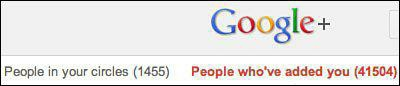
\includegraphics{images/size-of-audience-in-google-plus-circles.png}
    }
    \captionsource{Ilość osób w~kręgach}{\parencite[s.96]{Brogan12}}
    \label{fig:size-of-audience-in-google-plus-circles}
\end{figure}

Pierwszą z~nich jest \emph{liczba osób w~Twoich kręgach} oraz \emph{osoby, które dodały Cię do swoich kręgów}. Jak na razie sprawa jest bardzo prosta i~intuicyjna. Jednak Google w~budowaniu sieci połączeń nałożył pewne restrykcje ograniczając liczbę osób we własnych kręgach do 5000 i~jest to najważniejsza grupa z~punktu widzenia prowadzenia profilu. Druga grupa (tj. osoby, które  dodały nasz profil do swoich kręgów) może mieć nieograniczone rozrastanie i~można tą grupę określić w~skrócie jako widownie. 

Na temat różnych strategii budowania widowni naszego kanału wspomnianych nieco wyżej można poświęcić osobną książkę. Dla zainteresowanych polecam pozycję \parencite{Brogan12}.


\subsubsection{Słuchaj oraz wypowiadaj się}
\lipsum[24]

To o czym będzie mowa w~to między innymi:

\begin{itemize}
\item Opinie;
\item Hangouts;
\end{itemize}

\lipsum[67-70]

\lipsum[100-101]

%############################################################################

\subsubsection{Dziel się, ucz się i~odkrywaj}
Jak każde medium społecznościowe umożliwianie interakcji i~integracji społeczności w~której się otacza jest jednym z~kluczowych funkcjonalności. 

Również Google+ umożliwia umieszczanie treści czy to w~postaci grafiki, jeśli jest ukazać przykładowe nowe danie w~menu, czy tekstu, w~przypadku ciekawej wypowiedzi np. w~gazecie, czy wideoklipu ukazującego nowo otwartą salę w~restauracji. Może być również dowolnym połączeniem tych elementów. Oczywiście, podane przykłady nawiązują do restauracji, jednak są to tylko pewne punkty odniesienia, które równie dobrze mogą znaleźć zastosowanie w~innych branżach.

Sama idea dzielenia się informacjami jest bardzo pozytywnym przejawem i~powinno się zachęcać do udostępniania nowych ciekawych informacji. Oczywiście nie można ujawniać wszystkiego w~działaniu firmy, ale przykładowo podzielenie się pysznym świątecznym przepisem naszego szefa kuchni wraz ze zdjęciem jest informacją wartościową, pozytywnie wpływającą na klienta/użytkownika. Wartościową, ponieważ firma jest pewna tego co robi dając jasny przekaz klientowi, natomiast klient może we własnym zakresie poeksperymentować z~dostarczoną informacją, a dzięki przepisowi szefa kuchni sama może się poczuć jak szef kuchni \parencite[s.101]{Brogan12}, czyniąc klienta bohaterem.

Użytkownicy i~klienci bardzo często zwracają cenne informacje i~uwagi z~przepisów umieszczonych na stronie. Umieszczają swoje wrażenia, wyrażając swój zachwyt lub ubolewanie, a co wiąże się z~opiniami oraz dalszym ,,automatycznym'' promowaniem firmy w~świat --- bez udziału pracowników, czy wkładu finansowego.

%############################################################################

\subsubsection{Ścisła kontrola pod czujnym okiem producenta}
Firma Google oferuje jeszcze kilka bardzo ważnych informacji z~punktu widzenia promocji, w~tym szeroko rozumianego SEO (ang. \textit{Search Engine Optimalization}).

W tym miejscu można wyróżnić \parencite{url:google-plus-firmy-panel-google}: 

\begin{itemize}
\item Podgląd na najpopularniejsze wyszukiwania w~Google związane z~firmą;
\item Informacja o tym, na ile Twój profil Google+ jest kompletny;
\item Wyświetlanie statystyk społecznościowych, aby lepiej ocenić popularność wpisów w~Google+;
\item Zarządzać reklamami, w~tym także tymi w~AdWords Express.
\end{itemize}

Nasuwa się więc pytanie --- \emph{dlaczego akurat SEO w~promocji na portalach społecznościowych?}

Otóż w~przypadku produktu jakim jest Google+ i~najczęściej wykorzystywanej przez Polaków wyszukiwarki Google (ponad 96\%) istnieje pewna mało sprecyzowana korelacja między wynikami wyszukiwania w~wyszukiwarce Google, a promocją firmy w~sieci. 

\begin{figure}[!h]
\centering
    \scalebox{0.32}
    {
        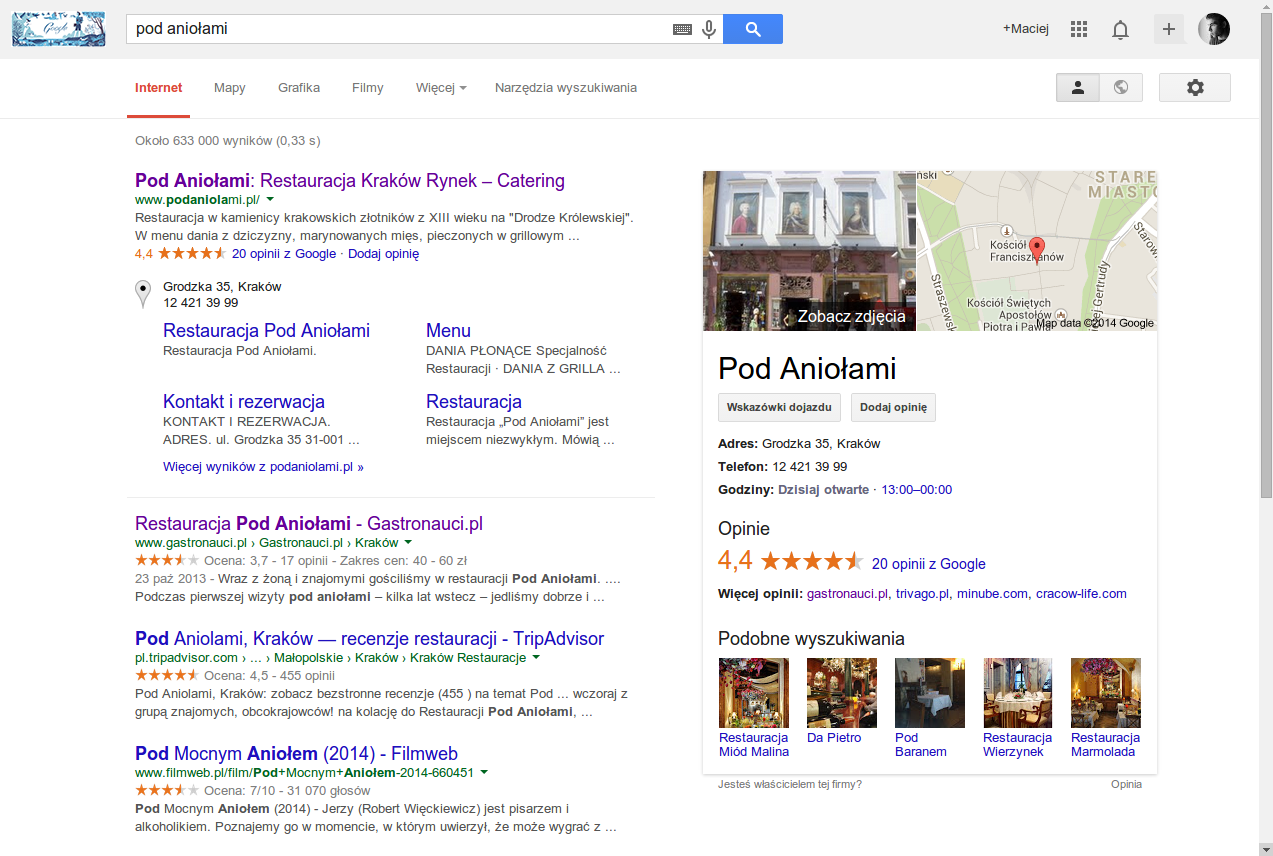
\includegraphics{images/search-result-company-in-google-search-engine.png}
    }
    \captionsource{Wyszukiwanie firmy w~wyszukiwarce Google}{Opracowanie własne.}
    \label{fig:search-result-company-in-google-search-engine}
\end{figure}

Trudno spekulować czy nawet pokusić się o stwierdzenie, że posiadanie konta w~Google+ ma jakiś wpływ na czynniki biorące udział w~wyrzucaniu wyników wyszukiwania\footnote{Według nieoficjalnych informacji ogólna liczba czynników biorących udział w~budowaniu zestawienia wyników wyszukiwarki Google przekracza 200 i~nieustannie wzrasta.} w~wyszukiwarce tego samego producenta. Wiadome jest jednak to, że firma bardzo mocno strzeże algorytmu odpowiedzialnego za sortowanie wyników. Jednak dostosowanie profilów (lub jak kto woli stron) budowanych przez usługę Google+ jest z~pewnością traktowane jest z~dużo większymi przywilejami niż wszystko inne\footnote{Wyjątkiem od tej reguły może okazać się marketing SEO, a firma Google uzyska odpowiednia opłatę np. poprzez system AdWords jako odrębna usługa służąca promocji firm konkurencyjnych w~wyszukiwarce Google --- lecz to jedynie spekulacje, ponieważ nie znając dokładnych zasad, które dodatkowo nie są precyzowane jednoznacznie przez producenta, ciężko określić czy takie działania rzeczywiście miałyby miejsce.}.

Bardzo dobrym dowodem, obserwowalnym gołym okiem wpływającym na opłacalność posiadania profilu w~Google+ i~osób korzystających z~wyszukiwarki tego samego producenta jest rysunek \ref{fig:search-result-company-in-google-search-engine}, który jednoznacznie ukazuje z~prawej strony ekranu ,,promocję'' firmy. Oczywiście szereg prawdopodobnych czynników takich jak korzystanie z~wyszukiwarki posiadając konto w~systemie Google (po zalogowaniu), lokalizacja wyszukiwania, czy rodzaj zapytania kierowanego do wyszukiwarki mogą mieć rażące znaczenie w~pozycjach wyszukiwarki\footnote{Nie są to oczywiście wszystkie możliwe warianty, które należy wziąć pod uwagę. Możliwe jest również to, że firma, która w~niniejszym opracowaniu posłużyła jako element modelu oprócz profilu Google+ stosuje reklamę w~AdWords (dzięki temu ma trafniejsze wyniki po wpisaniu określonych fraz). To trudno przewidzieć lub dowiedzieć się bez konsultacji z~firmą. Jednak niepodważalnym jest to, iż wyświetlane dane (np.: opinie) pochodzą z~serwisu Google+ lub na nim bazują.}, lecz jak widać na pierwszej stronie wyników można uzyskać chwytliwą promocję personalizując swoje dane na profilu Google+ nieodpłatnie. Takie działanie można określić skuteczną, dodatkową promocja w~ramach posiadania profilu Google+.\\

\hfill Autor: \textit{Maciej Sypień}
\section{Podsumowanie}
\label{sec:podsumowanie}

\lipsum[21-29]

\listoffigures
\clearpage
\printbibliography

\end{document}